% Prof. Dr. Ausberto S. Castro Vera
% UENF - CCT - LCMAT - Curso de Ci\^{e}ncia da Computa\c{c}\~{a}o
% Campos, RJ,  2023
% Disciplina: An\'{a}lise e Projeto de Sistemas
% Aluno: 

\chapterimage{planejamento.png} % Table of contents heading image
\chapter{Etapa de Planejamento}

Neste capítulo será apresentado como funcionará as etapas de planejamento e projeção do futuro do projeto do sistema DSS. Como a necessidade do sistema em questão para uma empresa, cronograma, custos e benefícios do sistema e entre outras questões que serão apresentadas nesse capítulo.


\section{Solicita\c{c}\~{a}o do Sistema}
%%%%%%%%%%%%%%%%%%%%%%%%%%%%%%%
\begin{itemize}
	\item \textbf{Responsável Pelo Projeto Do Sistema:} Gabriel Costa Fassarella.
	
	\item \textbf{Necessidade da empresa:} No cenário de negócios altamente competitivo e globalizado do mundo contemporâneo, a entrega eficiente de produtos e serviços desempenha um papel fundamental na satisfação do cliente e na vantagem competitiva de uma empresa. Para alcançar esse objetivo, muitas empresas devem recorrer a sistemas computacionais de monitoramento de entregas em tempo real. Esses sistemas oferecem uma série de benefícios que não apenas melhoram a experiência do cliente, mas também otimizam a eficiência operacional e reduzem os custos. Esses sistemas oferecem uma visão abrangente de toda a cadeia de suprimentos e logística. Eles permitem otimizar rotas de entrega, alocar tarefas de forma eficiente e monitorar o desempenho dos motoristas e veículos em tempo real. Isso resulta em economia de custos significativa, pois reduz o consumo de combustível, diminui o desgaste dos veículos e permite que mais entregas sejam feitas em menos tempo. Todo esse cenário acarreta na melhoria significativa da satisfação do cliente, visto que estes valorizam a transparência. Com um sistema de rastreamento em tempo real, os clientes podem acompanhar o status de suas entregas, receber estimativas precisas de chegada e até mesmo ajustar suas programações com base nessas informações.  
	
	\item \textbf{Requisitos de negócio:} 
	\begin{itemize}
		\item \textbf{Rastreamento:} A capacidade de rastrear entregas em tempo real, pode fornecer não apenas aos clientes, mas também as equipes de logística informações precisas sobre a localização e o status das encomendas.
		
		\item \textbf{Otimização:} Com isso, a empresa poderá otimizar as rotas de entrega, garantindo que os motoristas optem por rotas mais eficientes, levando em consideração o tráfego e outras variáveis que podem influenciar, como horários de entrega e restrições de veículos.
		
		\item \textbf{Gestão da Frota:} A empresa pode monitorar o desempenho de seus veículos e motoristas em tempo real, garantindo que os recursos sejam alocados de forma adequada, a manutenção seja programada e os motoristas estejam seguindo as diretrizes estabelecidas.
	\end{itemize}

	\item \textbf{Valor agregado:} 
	\begin{itemize}
		\item \textbf{Redução de Custos:} A otimização de rotas, a manutenção preventiva e a alocação eficiente de recursos ajudam a reduzir os custos operacionais, como combustível, manutenção de veículos e horas de trabalho extras.
		
		\item \textbf{Aumento da Eficiência Operacional:} O sistema permite otimizar rotas de entrega, reduzir tempos de viagem e economizar recursos, resultando em operações mais eficientes e econômicas.
		
		\item \textbf{Maior Segurança:} A capacidade de monitorar a localização dos veículos e das cargas ajuda a prevenir roubos e aumenta a segurança dos motoristas, além de melhorar a capacidade de resposta em situações de emergência.
		
		\item \textbf{Melhoria da Satisfação do Cliente:} A capacidade de oferecer aos clientes o rastreamento em tempo real de suas entregas cria uma experiência mais satisfatória. Os clientes se sentem mais informados e no controle, reduzindo a ansiedade relacionada à entrega.
	\end{itemize}
\end{itemize}

\section{Custos: Desenvolvimento e Operacional} 
%%%%%%%%%%%%%%%%%%%%%%%%%%%%%%%
Os principais custos relacionados ao sistema são: 
\begin{itemize}
	\item \textbf{Desenvolvimento:}
	\begin{itemize}
		\item \textbf{Desenvolvimento/Aquisição do Software:}  Se a empresa optar por desenvolver seu próprio sistema, haverá custos associados ao desenvolvimento de software, incluindo a contratação de desenvolvedores e o tempo de desenvolvimento. Caso escolha um sistema pronto, haverá custos de licenciamento e aquisição.
		
		\item \textbf{Hardware para Veículos:} dispositivos de rastreamento GPS em veículos.
		
		\item \textbf{Conectividade e Comunicação:} Custos de dados móveis e comunicação para transmitir informações em tempo real entre os veículos e o sistema central.
		
		\item \textbf{Hardware e Infraestrutura:} Os custos de hardware incluem servidores, dispositivos de rastreamento GPS, sensores, dispositivos móveis para motoristas, entre outros.
	\end{itemize}
	\item \textbf{Implementação:}
	\begin{itemize}
		\item \textbf{Treinamento e Implantação:} Os custos de treinamento da equipe e a implantação do sistema nas operações da empresa.
		
		\item \textbf{Manutenção:} É importante considerar os custos contínuos de manutenção do sistema, incluindo atualizações de software, suporte técnico e correções de bugs.
	\end{itemize}
\end{itemize}

\section{Benef\'{\i}cios}
%%%%%%%%%%%%%%%%%%%%%%%%%%%%%%%
Os benefícios relacionados ao sistema podem ser muitos, tanto tangíveis quanto intangíveis.

       \subsection{Benef\'{\i}cios Tang\'{\i}veis}
		\begin{itemize}
			\item \textbf{Melhoria da eficiência operacional:} O rastreamento em tempo real permite que as empresas monitorem a localização e o status de ativos, veículos ou pessoas, o que pode resultar em uma gestão mais eficiente de recursos.
			
			\item \textbf{Redução de custos:}  Ao otimizar o uso de recursos e reduzir o desperdício, as empresas podem economizar dinheiro em combustível, manutenção, mão-de-obra e outros custos operacionais.
			
			\item \textbf{Aumento da segurança:} O rastreamento em tempo real pode ser utilizado para monitorar a segurança de pessoas e produtos. Isso pode ajudar a prevenir roubos e fornecer respostas mais rápidas em casos de emergência.
		\end{itemize}

       \subsection{Benef\'{\i}cios Intang\'{\i}veis}
		\begin{itemize}
			\item \textbf{Visibilidade e transparência:} A capacidade de monitorar operações em tempo real pode aumentar a transparência nas operações da empresa.
			
			\item \textbf{Aprimoramento da reputação da marca:} Empresas que demonstram comprometimento com a eficiência, segurança e responsabilidade através do rastreamento em tempo real podem construir uma reputação positiva no mercado.
			
			\item \textbf{Maior confiabilidade e credibilidade:} As empresas que utilizam sistemas de rastreamento em tempo real podem ganhar a confiança de clientes, investidores e parceiros comerciais, demonstrando um compromisso com a qualidade, segurança e eficiência.
		\end{itemize}

\section{An\'{a}lise de Custos e Benef\'{\i}cios}
%%%%%%%%%%%%%%%%%%%%%%%%%%%%%%%
Analisando todos os custos benefícios do sistema, conclui-se a necessidade de um sistema de monitoramento em tempo real, devido a necessidade de uma melhor gestão das entregas com o intuito de reduzir custos, otimizar o sistema de entregas e junto com isso, trazer uma melhor experiência ao cliente.




\section{Estudo de Viabilidade}
%%%%%%%%%%%%%%%%%%%%%%%%%%%%%%%
	Nesta seção será abordado o estudo de viabilidade do sistema: o quão viável é para faze-lo e se vale a pena projeta-lo.

       \subsection{Calend\'{a}rio }
		\begin{itemize}
			\item \textbf{Início do Projeto:} 09/02/2024
			
			\item \textbf{Planejamento do Projeto:} 09/02/2024 a 03/04/2024
			
			\item \textbf{Análise do Sistema:} 03/04/2024 a 05/07/2024
			
			\item \textbf{Implementação do Projeto:} 05/07/2024 a 15/12/2024
			
			\item \textbf{Fim do Projeto:} 15/12/2024 
		\end{itemize}
       \subsection{Cronograma }
% TODO: \usepackage{graphicx} required
\begin{figure}[H]
	\centering
	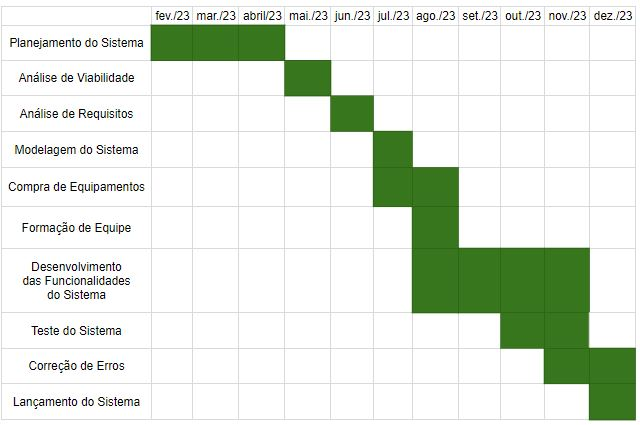
\includegraphics[width=0.8\linewidth]{Pictures/Cronograma}
	\caption{}
	\label{fig:cronograma}
\end{figure}

       \subsection{Or\c{c}amento }
       Nesta seção, será apresentado um orçamento para a produção do sistema computacional.

		Orçamento 1:
		% TODO: \usepackage{graphicx} required
		\begin{figure}[H]
			\centering
			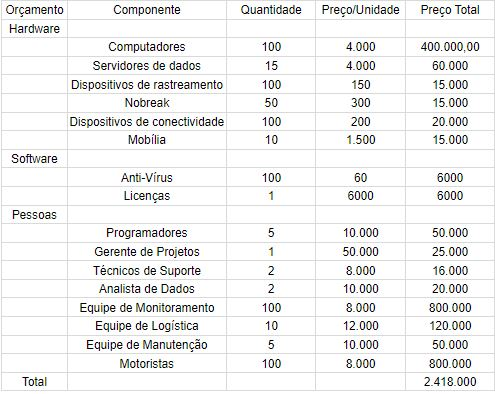
\includegraphics[width=0.7\linewidth]{Pictures/Orc}
			\caption{}
			\label{fig:orc}
		\end{figure}
	
		Orçamento 2:
		% TODO: \usepackage{graphicx} required
		\begin{figure}
			\centering
			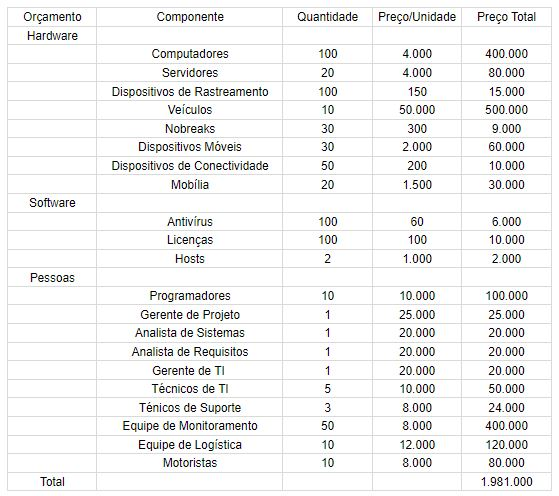
\includegraphics[width=0.7\linewidth]{Pictures/Orc2}
			\caption{}
			\label{fig:orc2}
		\end{figure}

       \subsection{Resumo e Recomenda\c{c}\~{o}es}

       Considerando os custos não muito elevados e curto tempo de produção do sistema computacional de forma completa e funcional, visando uma otimização do sistema de entregas da empresa, é sim viável o desenvolvimento do sistema D.S.S.
       
       Recomenda-se a utilização de rigorosos sistemas de segurança, visto que o vazamento de dados de clientes podem trazer inúmeros problemas a empresa, além disso o treinamento e documentação é essencial para o funcionamento do sistema D.S.S de maneira totalmente efetiva. Outro fator é criar um sistema com boa escalabilidade, visto que o fluxo de dados presente no sistema é extremamente alto, por isso garantir a escalabilidade é essencial para que o sistema funcione de maneira correta e completamente efetiva.
